\section{Linear System Identification}
\label{sec:sysid}

%% Overview of this section
Any finite-dimensional nonlinear dynamical system has an equivalent infinite-dimensional linear representation in the space of real-valued functions of the system's state \cite{mauroy2016linear} \Ram{cite a theorem.}.
In this function space, the (linear) Koopman Operator describes the flow of functions along trajectories of the system.
% The dual of the Koopman operator, the Perron-Frobenius operator, describes the dynamics of the system...
While it is not possible to numerically represent the infinite-dimensional Koopman operator, it is possible to represent its projection onto a finite-dimensional subspace as a matrix.
% Our goal is to construct models in this subspace in the form of a controlled linear dynamical system
% \begin{align}
%     \psi_{k+1} &= A \psi_{k} + B u_{k} \\
%     y_{k} &= C \psi_{k}
% \end{align}
% where $z$ is ... , $u$ is the input, and $y$ is the output of the system.
We will show that for a given choice of basis functions, a \emph{lifted} linear dynamical system model can be extracted directly from the matrix approximation of the Koopman operator.
% As desired, system representations of this form lend themselves to linear control methods.

The remainder of this sections outlines the approach for constructing the Koopman operator approximation and the linear system representation from data.
Section \ref{sec:mpc} illustrates how this model can be incorporated into a model predictive control algorithm.

%% Overview of the Koopman operator and how it represents dynamical systems
\subsection{Koopman Representation of a Dynamical System}

%% System representation in state space
Consider a dynamical system
\begin{align}
    \dot{x}(t) &= F (x(t)) \\
    \label{eq:nlsys}
\end{align}
where $x(t) \in \Real^n$ is the state of the system at time $t$, and ${F}$ is a continuously differentiable function.
Denote by $\phi(t,x_0)$ the solution to \eqref{eq:nlsys} at time $t$ when beginning with the initial condition $x_0$ at time $0$ \Ram{for simplicity we may want to write this down as a function with a domain and range and then describe what it means at a specific argument}.
For simplicity, we denote this map, which is referred to as the \emph{flow map}, by $\phi_t (x_0)$ instead of $\phi (t, x_0)$

%% System representation in the space of observables
The system can be lifted to an infinite dimensional function space $\mathcal{F}$ composed of all square integrable real-valued functions with compact domain $X \subset \Real^n$.
Elements of $\mathcal{F}$ are called \emph{observables}.
In $\mathcal{F}$, the flow of the system is characterized by the set %semigroup 
of Koopman operators 
$U_t : \mathcal{F} \to \mathcal{F}$, for each $t \geq 0$,
which describes the evolution of the observables ${f \in \mathcal{F}}$ along the trajectories of the system according to the following definition:
\begin{align}
    U_t f = f \circ \phi_t      
    % && \forall f \in \F, t \geq 0
    \label{eq:koopman}
\end{align}
As desired, $U_t$ is a linear operator even if the system \eqref{eq:nlsys} is nonlinear, since for $f_1, f_2 \in \mathcal{F}$ and $\lambda_1, \lambda_2 \in \Real$
\begin{align}
    \begin{split}
    U_t (\lambda_1 f_1 + \lambda_2 f_2) &= \lambda_1 f_1 \circ \phi_t + \lambda_2 f_2 \circ \phi_t \\
    &= \lambda_1 U_t f_1 + \lambda_2 U_t f_2.
    \end{split}
\end{align}
Thus the Koopman operator provides a linear representation of the flow of a nonlinear system in the infinite-dimensional space of observables (see Fig. \ref{fig:overview}) \cite{budivsic2012applied} \Ram{you need to say something more explicit here. While $\phi$ describes how an initial condition flows according to the ODE, the Koopman operator describes how a function evolves according to the ODE. Notice that one can go back and forth between the representations...}.


%% Koopman-based system identification (consult ICRA paper)
\subsection{Identification of Koopman Operator}
\label{sec:koopid}

Since the Koopman operator is an infinite-dimensional object, it cannot be represented by a finite-dimensional matrix. 
Therefore, we settle for the projection of the Koopman operator onto a finite-dimensional subspace.
Using a modified version of the Extended Dynamic Mode Decomposition (EDMD) algorithm \cite{williams2015data} originally presented in \cite{mauroy2016linear} and \cite{mauroy2017koopman}, we identify a finite-dimensional approximation of the Koopman operator via linear regression performed on observed data.

Define ${\bar{\mathcal{F}} \subset \mathcal{F}}$ to be the subspace of $\mathcal{F}$ spanned by ${N>n}$ linearly independent basis functions, 
${ \{ \psi_k : \Real^n \to \mathcal{R}_k \subseteq \Real \}_{k=1}^N}$ \Ram{what is $ \mathcal{R}_k$?}\Dan{it's just to show that the range of each observable need not be all of the reals}
\footnote{To see why $\psi_k$ may not map to all of $\Real$, consider e.g. the basis function $\psi_k(x) = \sin{(x)}$ which maps $x$ only onto $[-1,1] \subset \Real$.}.
Also let the first $n$ basis functions be defined
\begin{align}
    &\psi_k(x) = x_k , && k = 1, \dots , n
    \label{eq:xinpsi}
\end{align}
where $x_k$ denotes the $k^{th}$ element of $x$ \Ram{this is bad notation. You wnat it to be subscript instead of superscript.}\Dan{subscript already means something else...}.
Any observable $\bar{f} \in \bar{\mathcal{F}}$ can be expressed as a linear combination of elements of these basis functions
\begin{align}
    \bar{f} &= \theta_1 \psi_1 + \cdots + \theta_N \psi_N
    \label{eq:fexpanded}
\end{align}
where each $\theta_i \in \Real$.
For convenience in presentation, we introduce the vector of coefficients ${\theta = [ \theta_1 \,  \cdots \, \theta_N ]^\top}$ and the \emph{lifting function} ${\psi : \Real^n \to \mathcal{M} \subset \Real^N}$ defined as:
\begin{align}
    \psi(x) &:= \begin{bmatrix} \psi_1 (x) & \cdots & \psi_N (x) \end{bmatrix}^\top
    \label{eq:lift}
\end{align}
where $\mathcal{M} = \mathcal{R}_1 \times \cdots \times \mathcal{R}_N$.
By \eqref{eq:fexpanded} and \eqref{eq:lift}, $\bar{f}$ evaluated at a point $x$ is given by
% Note that $\bar{\theta}$ provides a vector representation for ${ \bar{f} \in \bar{\mathcal{F}} }$, and $\bar{f}$ evaluated at a point $x$ is given by
% Then, $\bar{f} \in \bar{\mathcal{F}}$ can be expressed concisely as
\begin{align}
    \bar{f}(x) &= \theta^\top \psi (x)
    \label{eq:fvec}
\end{align}
We therefore refer to $\psi(x)$ as the \emph{lifted state}, and $\theta$ as the \emph{vector representation} of $\bar{f}$.

Given this vector representation for observables, a linear operator $L : \bar{\mathcal{F}} \to \bar{\mathcal{F}}$ can be represented as an ${N \times N}$ matrix. 
We denote by $\bar{U}_t \in \Real^{N \times N}$ the approximation of the Koopman operator in $\bar{\mathcal{F}}$, which operates on observables via matrix multiplication:
\begin{align}
    \bar{U}_t \theta = \theta'
\end{align}
where $\theta , \theta'$ are each vector representations of observables in $\bar{\mathcal{F}}$.
%% Pulled straight from ICRA paper below this line
Our goal is to find a $\bar{U}_t$ that describes the action of the infinite dimensional Koopman operator $U_t$ as accurately as possible in the $L^2$-norm sense on the finite dimensional subspace $\bar{\mathcal{F}}$  of all observables.
Therefore, to perfectly mimic the action of $U_t$ acting on an observable ${f \in \bar{\mathcal{F}} \subset \mathcal{F}}$, according to \eqref{eq:koopman} the following should be true for all $x$ \Ram{super confused what the relationship between the first and second equation below is supposed to be. I agree that the second implies the first, but i'm not sure why you are showing the first equation}\Dan{should be clear now. We should discuss how to cut this down.}
\begin{align}
    \bar{U}_t \bar{f}(x) &= \bar{f} \circ \phi_t (x) \\
    ( \bar{U}_t {\theta} )^\top {\psi}(x) &=
    {\theta}^\top {\psi} \circ \phi_t(x) \\
    \bar{U}_t^\top \psi(x) &= {\psi} \circ \phi_t(x)
    \label{eq:UbarEq}
\end{align}
Since this is a linear equation, it follows that for a given ${x \in \Real^n}$, solving \eqref{eq:UbarEq} for $\bar{U}_t$ yields the best approximation of $U_t$ on $\bar{\mathcal{F}}$ in the $L^2$-norm sense \Ram{cite a result}:
\begin{align}
    \bar{U}_t = \left( {\psi}(x)^\top \right)^\dagger {\psi}( \phi_t(x) )^\top
    \label{eq:Uapprox}
\end{align}
where superscript $\dagger$ denotes the least-squares pseudoinverse.

%% How this is done on our system
To approximate the Koopman operator from a set of experimental data, we take $K$ discrete state measurements 
in the form of so-called ``snapshot pairs'' ${ \{ a_k , b_k \} \in \Real^{n \times 2} }$ where
% with sampling period $T_s$. We separate the data into a set of $K$ so-called ``snapshot pairs'' of the form ${ \{ a_k , b_k \} \in \Real^{n \times 2} }$ where
\begin{align}
    a_{k} &= x_{[k]} \\
    b_{k} &= \phi_{T_s} (x_{[k]}) + \sigma_k,
    \label{eq:ab}
\end{align}
$\sigma_k$ denotes measurement noise, and $T_s$ is the sampling period which is assumed to be identical for all snapshot pairs.
% For our basis of $\bar{\mathcal{F}}$, we choose the basis of monomials of $x$ with total degree less than or equal to $w$, which implies ${N=(n+m+w)!/\left((n+m)!w!\right)}$ \cite[Section III]{mauroy2016linear}. 
We then lift all of the snapshot pairs according to \eqref{eq:lift} and compile them into the following ${K \times N}$ matrices:
\begin{align}
    &\Psi_a := \begin{bmatrix} {\psi}(a_1)^\top \\ \vdots \\  {\psi}(a_K)^\top \end{bmatrix}
    &&\Psi_b := \begin{bmatrix} {\psi}(b_1)^\top \\ \vdots \\  {\psi}(b_K)^\top \end{bmatrix}
    \label{eq:Psi}
\end{align}
$\bar{U}_{T_s}$ is chosen so that it yields the least-squares best fit to all of the observed data, which, following from \eqref{eq:Uapprox}, is given by 
\begin{align}
    \bar{U}_{T_s} &:= \Psi_a^\dagger \Psi_b.
\end{align}

%% Incorporating Delays
Sometimes a more accurate model can be attained by incorporating delays into the set of snapshot pairs. To do so we define the snapshot pairs as
\begin{align}
    a_k &= \begin{bmatrix} x_{[k]}^\top, & x_{[k-1]}^\top, & \cdots, & x_{[k-d]}^\top \end{bmatrix}^\top \\
    b_k &= \begin{bmatrix} \left( \phi_{T_s} (x_{[k]}) + \sigma_k \right)^\top, & x_{[k]}^\top, & \cdots, & x_{[k-d+1]}^\top \end{bmatrix}^\top
\end{align}
where $d$ is the number of delays.
We then modify the domain of the lifting function such that $\psi : \Real^{n+nd} \to \Real^{N}$ to accommodate the larger dimension of the snapshot pairs.
% without input delays or $\Real^{n+nd} \times \Real^{md}$ with input delays.
For a system with inputs, we can also include input delays by appending them in a similar fashion \Ram{I think you mean for systems with input you can include input into the state just as you did with the delays?}.
Once these snapshot pairs have been assembled, the model identification procedure is identical to the case without delays.


%% Koopman representation of controlled dynamical system
\subsection{Building Linear System from Koopman Operator}

We are interested in using the Koopman operator \Ram{are you capitalizing operator or not? Sometimes you are, sometimes you aren't.} to construct linear models for dynamical systems with inputs of the form \Ram{why? I think motivating why these models are particularly useful may be a good strategy. Like maybe start with a brief description about how linear MPC works and then dive into these kind of models?}
\begin{equation}
\begin{aligned}
    z_{[k+1]} &= A z_{[k]} + B u_{[k]} \\
    y_{[k]} &= C z_{[k]}
    \label{eq:linSys}
\end{aligned}
\end{equation}
where $x_{[0]}$ is the initial condition in state space, $z_0 = \psi(x_{[0]})$, and $u_{[k]} \in \Real^m$ is the input \Ram{I only see $u_k$ not $u$}.
Specifically, we desire a representation in which (non-lifted) inputs appear \emph{linearly}, because models of this form are amenable to linear feedback control methods.
We construct a model of this form by first applying the system identification method of Section \ref{sec:koopid} to the modified snapshot pairs \Ram{probably easier if you can refer to a specific equation}
% \begin{align}
%     \alpha_k &= \begin{bmatrix} \psi(a_k)^\top & u_k^\top \end{bmatrix} \\
%     \beta_k &= \begin{bmatrix} \psi(b_k)^\top & u_k^\top \end{bmatrix} 
% \end{align}
\begin{align}
    &\alpha_k = \begin{bmatrix} \psi(a_k) \\ u_{[k]} \end{bmatrix} 
    &&\beta_k = \begin{bmatrix} \psi(b_k) \\ u_{[k]} \end{bmatrix} 
\end{align}
The input $u$ is not lifted so that it appears linearly in the resulting model.
With these pairs, we define the following ${K \times (N + m)}$ matrices:
\begin{align}
    &\Gamma_\alpha = \begin{bmatrix} \alpha_1^\top \\ \vdots \\  \alpha_K^\top \end{bmatrix}
    &&\Gamma_\beta = \begin{bmatrix} \beta_1^\top \\ \vdots \\  \beta_K^\top \end{bmatrix}
    \label{eq:Gamma}
\end{align}
and solve for the corresponding Koopman operator according to \eqref{eq:Uapprox}
\begin{align}
    \bar{U}_{T_s} &:= \Gamma_{\alpha}^\dagger \Gamma_\beta.
    \label{eq:koopGamma}
\end{align}
Note that by \eqref{eq:UbarEq} and \eqref{eq:koopGamma} the transpose of this Koopman matrix is the best approximation of a transition matrix between the elements of snapshot pairs in the $L^2$-norm sense \Ram{cite a result}
\begin{align}
    \bar{U}_{T_s}^\top 
    \begin{bmatrix} \psi(a_k) \\ u_{[k]} \end{bmatrix} &\approx
    \begin{bmatrix} \psi(b_k) \\ u_{[k]} \end{bmatrix},
\end{align}
and we desire the best $A,B$ matrices such that
\begin{align}
    A \psi(a_k) + B u_k &\approx \psi(b_k)
    \label{eq:linSys_psi}
\end{align}
Therefore, the best $A$ and $B$ matrices of \eqref{eq:linSys} are embedded in $\bar{U}_{T_s}^\top$ and can be isolated by partitioning it as follows:
\begin{align}
    \bar{U}_{T_s}^\top &= 
    \begin{bmatrix} 
        A_{N \times N} &
        B_{N \times m} \\
        O_{m \times N} &
        I_{m \times m}
    \end{bmatrix}
    \label{eq:AB}
\end{align}
where $I$ denotes an identity matrix, and $O$ denotes a zero matrix \Ram{you have not explained what the subscripts mean.}.
The $C$ matrix is defined
\begin{align}
    C &= \begin{bmatrix} I_{n \times n} & O_{n \times (N-n)} \end{bmatrix}
\end{align}
since by \eqref{eq:xinpsi}, ${x = [ \psi_1(x) , \dots , \psi_n(x) ]}$.

% \begin{align}
%     z_{k+1} &= A z_k + B u_k
%     \label{eq:linSys}
% \end{align}

% \begin{align}
%     \begin{bmatrix} \psi(b_k) \\ u_k \end{bmatrix} &=
%     \begin{bmatrix} A_{N \times N} & B_{N \times m} \\ O_{m \times N} & I_{m \times m} \end{bmatrix} 
%     \begin{bmatrix} \psi(a_k) \\ u_k \end{bmatrix}
% \end{align}


%% Why should we use lasso instead of the least-squares solution
\subsection{Practical Considerations: Overfitting and Sparsity}

%% Need a way to deal with outliers
A pitfall of data-driven modeling approaches is the tendency to overfit.
While least-squares regression yields a solution that minimizes the total root-mean-square error (RMSE) with respect to the training data, this solution does not necessarily generalize well to new data since it has been shaped by noise and outliers in the training data.
To protect against overfitting in identifying $\bar{U}_{T_s}$, we utilize the $L^1$-regularization method of least absolute shrinkage and selection operator (LASSO):
%% Lasso optimization problem
\begin{equation}
\begin{aligned}
\hat{\vec{U}}_{T_s} &= 
& \text{arg}~\underset{ \vec{U}_{T_s} }{\text{min}}
& & || \vec{\Gamma}_\alpha \vec{U}_{T_s} - \vec{\Gamma}_\beta ||_2^2 + \lambda || \vec{U}_{T_s} ||_1
\label{eq:lasso}
\end{aligned}
\end{equation}
where $\lambda \in \Real^{+}$ is the weight of the $L^1$ penalty term, and $\vec{\cdot}$ denotes a vectorized version of each matrix with dimensions consistent with the stated problem \Ram{you may just want to use $\text{vec}(X)$ instead of the arrow}.
For $\lambda = 0$, \eqref{eq:lasso} provides the same unique least-squares solution as \eqref{eq:koopGamma}; as $\lambda$ increases it drives the elements of $\vec{U}_{T_s}$ to zero.
For an overview of the LASSO method and how to implement it, see \citet{tibshirani1996regression}.

%% Lasso promotes sparsity
The benefit of using $L^1$-regularization to reduce overfitting rather than $L^2$-regularization (e.g. ridge regression) is its ability to drive elements to zero (rather than just making them small).
This promotes sparsity in the resulting Koopman operator approximation (and consequently the $A$ and $B$ matrices).
Sparsity is a desirable trait because it reduces the computational cost of solving the optimization problems involved in model predictive control. 
As a consequence, control inputs can be calculated faster for models with sparser matrix representations, enabling higher bandwidth control.

%% The cost of sparsity, falling off the manifold
\Dan{Here things get dicey. Will need to be rewritten.}
While sparsity is desirable, it comes at a cost.
The lifting function $\psi$ maps from $\Real^n$ to $\mathcal{M}$, but $A\psi(x) + B u$ may not map onto $\mathcal{M}$.
If that is the case, if we try to simulate our linear model from an initial condition, it may leave the space of legitimate ``lifted states'' rather quickly and fail to predict behavior accurately.
We therefore desire the sparsest model that minimizes the distance from $\mathcal{M}$ at each iteration.
This can be accomplished by applying a projection operator at each time step.
The perfect projection operator $P$ should satisfy
\begin{align}
    P \left( A {\psi}(a_k) + B u_k \right) &= \psi(b_k)
\end{align}
for all $k$. 
If we compile the following $K \times N$ matrix,
\begin{align}
    &\Omega_a := \begin{bmatrix} \left( A {\psi}(a_1) + B u_1 \right)^\top \\ \vdots \\  \left( A {\psi}(a_K) + B u_K \right)^\top \end{bmatrix},
    \label{eq:Omega}
\end{align}
then the best projection operator in the $L^2$-norm sense based on our data is given by
\begin{align}
    P := \left( \Omega_{a}^\dagger \Psi_b \right)^\top.
\end{align}
The modified linear model is then 
\begin{align}
    z_{k+1} &= P \left( A z_k + B u_k \right)
    \label{eq:linSys_wP}
\end{align}

%% Why is this better/different than just doing least squares to begin with?
\Dan{Here I plan to explain why this is better than doing least-squares right off the bat: It still yields a sparser model of equal accuracy, even with the projection operator.}

%% FIGURE: Lifting and Projecting
\begin{figure}
    \centering
    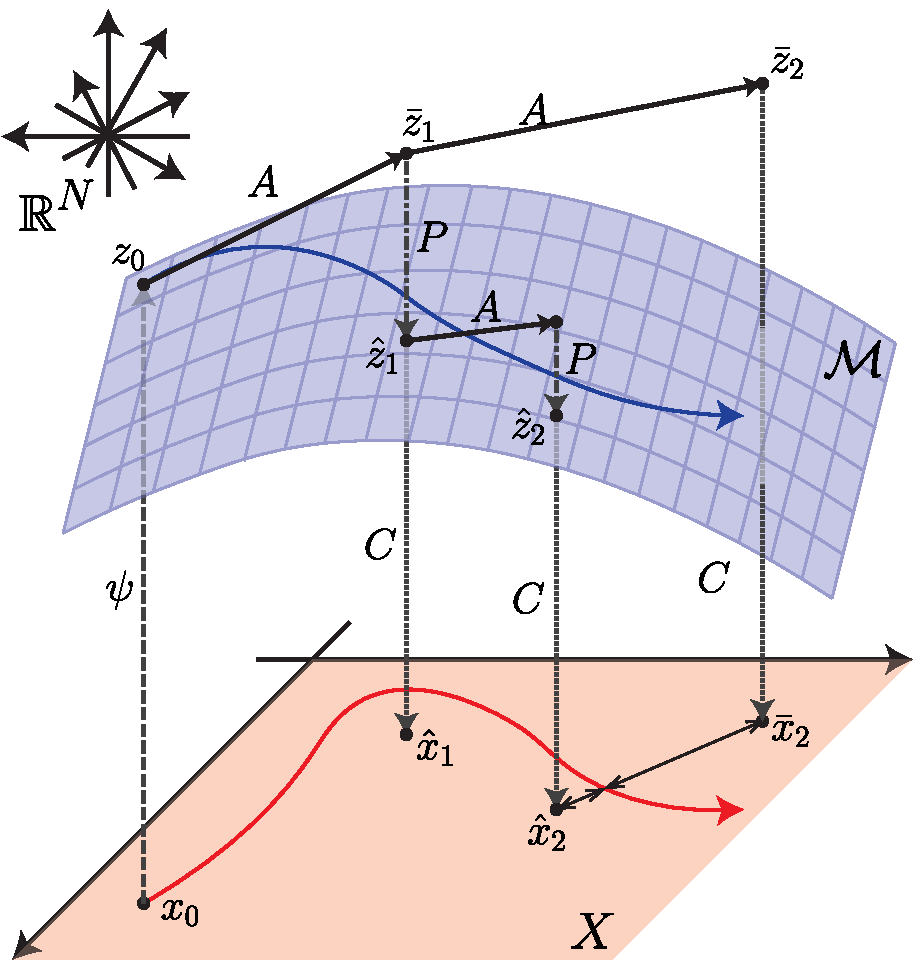
\includegraphics[width=0.9\linewidth]{figures/liftingManifold_v16.pdf}
    \caption{Caption}
    \label{fig:manifold}
\end{figure}